\section{Case Study: Qwen3.8-27B on DGX Spark}\label{sec:case}

The case study started with a practical question: on a DGX Spark, is there anything left to gain
in decode by fusing or tuning kernels? We first answered it by hand, with Nsight Systems traces,
arithmetic on weight sizes and the vLLM source; \sys{} came afterwards, as the tool we wished we
had, and reproduces the finding automatically. This section follows the order in which things
were found. All raw numbers and the scripts that produce them are in the repository under
\texttt{case-studies/gb10-qwen3.8-27b} and \texttt{paper/experiments}.

\paragraph{Setup.}
\Cref{tab:setup} lists the configuration. Each step runs four tokens per request through the main
model (one verified plus three drafts) and three draft steps of the MTP head. Unless stated
otherwise, measurements are taken over 40 steady-state steps at batch 1, after warm-up and graph
capture.

\begin{table}[t]
\centering\small
\begin{tabular}{@{}ll@{}}
\toprule
Machine & NVIDIA DGX Spark: GB10 (sm\_121, 48 SMs, 24\,MiB L2), 121\,GB unified LPDDR5x \\
Engine & vLLM 0.31.0 (main measurements), 0.34.0 and main (comparison); CUDA graphs \\
Model & Qwen3.8-27B, NVFP4 checkpoint (NVFP4 MLP in layers 0--55, FP8 elsewhere) \\
Architecture & 64 layers: 48 Gated DeltaNet, 16 full attention \\
Speculation & MTP head, 3 draft tokens \\
\bottomrule
\end{tabular}
\caption{Case study configuration.}\label{tab:setup}
\end{table}

\subsection{The ceiling}

The floor of a bandwidth-bound step is its bytes divided by the bandwidth the machine can
actually sustain, which is not the specification. A read-only kernel (\texttt{bench/bwtest.cu})
reaches 253.5\,GB/s; BabelStream~\cite{deakin2016babelstream} Dot reaches 253.0\,GB/s and Copy,
Mul, Add and Triad 248--252\,GB/s; a device-to-device \texttt{cudaMemcpy} reaches 243.0\,GB/s.
The specification is 273\,GB/s. We use 252\,GB/s throughout.

\subsection{The step}

\Cref{tab:step} gives the step books. Kernels are back to back: the gaps between them add up to
0.36\,ms per step, 0.3\%. Fusing kernels to remove launch gaps buys almost nothing on this
machine. Weight streaming runs at 84\% of the ceiling overall; at the ceiling the step would take
101\,ms instead of 121.

\begin{table}[t]
\centering\small
\begin{tabular}{@{}lr@{}}
\toprule
 & per step \\
\midrule
Wall time & 120.9\,ms \\
GPU busy & 120.5\,ms \\
Idle between kernels & 0.36\,ms (0.3\%) \\
Launches & 972 \\
Weight bytes streamed & 25.5\,GB \\
Effective bandwidth & 211\,GB/s (84\% of ceiling) \\
Floor at the ceiling & 101.1\,ms \\
\bottomrule
\end{tabular}
\caption{Step books at batch 1 (vLLM 0.31.0).}\label{tab:step}
\end{table}

\subsection{Where the bandwidth goes}

Most weight-streaming launches run at 85--96\% of the ceiling. Two items stand out. The
248k-vocabulary \texttt{lm\_head} (1.27\,GB in FP8) is read four times per step, once by the main
model and once by each draft step: 5.1\,GB and about 22\,ms, 18\% of the step time. And the output
projection of the Gated DeltaNet layers, \texttt{linear\_attn.out\_proj}, runs at 64\% of the
ceiling while every other FP8 projection of the main model runs at 85--91\%.

\subsection{Same kernel, same shape, different speed}\label{sec:split}

The GDN \texttt{out\_proj} and the attention \texttt{self\_attn.o\_proj} have weights of the same
shape ($6144\times5120$, FP8), both 4\,KB aligned, and are multiplied by the same CUTLASS kernel
with the same grid. The GDN one takes a median 194.6\,\textmu s over 1920 launches, the attention
one 147.3\,\textmu s over 640: 47\,\textmu s more per launch, 2.27\,ms per step. The kernel before
every slow launch that touched a cache region is the GDN decode kernel
(\texttt{gdn\_decode\_post\_conv\_mtp}, 1920 of 1920); before every fast launch it is attention
(640 of 640).

\paragraph{The weights are not the cause.}
\texttt{gemm\_isolation.py} runs the same vLLM GEMM op on the real weights at $M=4$, outside the
engine, with L2 swept by a read before each launch. GDN \texttt{out\_proj} of layers 0 and 1 and
attention \texttt{o\_proj} of layers 3 and 7 all take 147.5\,\textmu s (213\,GB/s).

\paragraph{Dirty lines are.}
Writing $N$\,MiB just before the GEMM, instead of reading, leaves $N$\,MiB of dirty
lines in L2 that must be written back while the GEMM streams its weight. The GEMM slows down
steadily with $N$ until L2 is full (\cref{fig:dirty}): 158.7\,\textmu s at 2\,MiB,
187.4\,\textmu s at 8\,MiB, 197.6\,\textmu s at 12\,MiB, 213.2\,\textmu s at 24\,MiB (the size of L2), and
215.0\,\textmu s at 32\,MiB. The in-engine 194.6\,\textmu s sits at about 11\,MiB on this curve.

\begin{figure}[t]
\centering
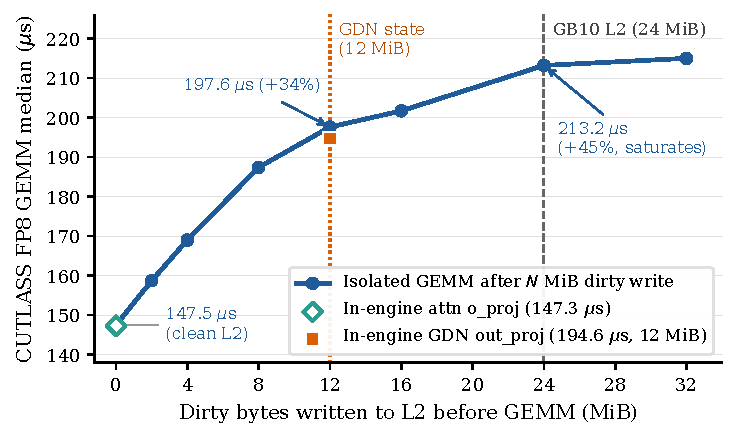
\includegraphics[width=0.75\linewidth]{figures/dirty_l2_sweep}
\caption{Mechanism, not fix: the $6144\times5120$ FP8 GEMM at $M=4$, isolated, slows down with the dirty bytes left in L2 before it. Markers: in-engine medians of attention \texttt{o\_proj} (no state written before it) and GDN \texttt{out\_proj} (placed at the 12\,MiB the GDN kernel writes).}\label{fig:dirty}
\end{figure}

\paragraph{Who writes them.}
The GDN decode kernel in vLLM keeps, for speculative decoding, the full recurrent state after
\emph{every} token of the step in a separate slot, so that rejected drafts can be rolled back. The
state is $48 \text{ heads} \times 128 \times 128$ in FP32, 3.15\,MB (3\,MiB) per position, 12.6\,MB (12\,MiB)
per layer for four positions. The stores land in L2, so the GDN kernel itself finishes in 41\,\textmu s; the
next weight-streaming kernel is \texttt{out\_proj}, which pays for the write-back. The next step
reads only the slot of the last accepted position.

\paragraph{Halving the state.}
If the mechanism is right, halving the bytes stored should shorten both kernels by a predictable
amount and leave the rest alone. vLLM can keep the recurrent state in BF16
(\texttt{--mamba-ssm-cache-dtype bfloat16}). The GB10 runs at a software power cap, and whole-step
times drift by as much as the effect, so we lock the clock at 2000\,MHz, alternate the two
configurations, and compare per-kernel books. \Cref{tab:bf16} shows that in both pairs the GDN
kernel halves and \texttt{out\_proj} drops by 14--17\,\textmu s, while \texttt{lm\_head}, which
follows neither, stays within its own drift. BF16 state changes numerics; it is a probe, not a fix.

\begin{table}[t]
\centering\small
\begin{tabular}{@{}lrrr@{}}
\toprule
Run & GDN decode & GDN \texttt{out\_proj} & \texttt{lm\_head} (control) \\
\midrule
A1 FP32 state & 41.2\,\textmu s & 192\,\textmu s & 5422\,\textmu s \\
B1 BF16 state & 21.6\,\textmu s & 175\,\textmu s & 5431\,\textmu s \\
A2 FP32 state & 40.6\,\textmu s & 190\,\textmu s & 5505\,\textmu s \\
B2 BF16 state & 21.7\,\textmu s & 176\,\textmu s & 5538\,\textmu s \\
\bottomrule
\end{tabular}
\caption{FP32 against BF16 recurrent state, alternating runs at a locked clock, batch 1. Medians per launch.}\label{tab:bf16}
\end{table}

\subsection{Removing the stores}

To bound what a fix can buy, we built the vLLM 0.31.0 GDN kernel as a standalone extension
(bitwise identical to the shipped op when compiled with \texttt{--use\_fast\_math}), added a switch
that keeps only the last position's store, and swapped it into the engine before graph capture.
This writes exactly as much state as a correct fix would; it is a performance probe only, since
after a rejected draft the state is wrong.

\Cref{tab:probe} shows the result. At batch 1 the stores fit in L2 and their cost lands on the
next GEMM: GDN decode drops from 40.8 to 23.3\,\textmu s and \texttt{out\_proj} from 194.6 to
162.7\,\textmu s, while the control \texttt{o\_proj} does not move. At batch 4 the stores are
48\,MiB per layer, twice the L2, and the GDN kernel itself stalls on DRAM writes: 267.6 against
83.7\,\textmu s. State traffic grows with the batch while weight traffic does not, so the saving
grows with load: 1\% of the step at batch 1, 6.8\% at batch 4.

At batch 1 the kernel-level saving is 2.4\,ms per step but the step gained only 1.2--1.4\,ms: in
that run the MLP \texttt{gate\_up} GEMMs were 4\% slower in every layer, GDN or attention, which
is consistent with power-cap drift. Per-kernel books make this visible; a step-time comparison
alone would have under-reported the effect by half.

\begin{table}[t]
\centering\small
\begin{tabular}{@{}lrrrr@{}}
\toprule
 & \multicolumn{2}{c}{batch 1} & \multicolumn{2}{c}{batch 4} \\
\cmidrule(lr){2-3}\cmidrule(lr){4-5}
 & all & last only & all & last only \\
\midrule
GPU busy per step & 120.9\,ms & 119.7\,ms & 131.7\,ms & 122.7\,ms \\
GDN decode & 40.8 & 23.3 & 267.6 & 83.7 \\
GDN \texttt{out\_proj} & 194.6 & 162.7 & 199.8 & 192.5 \\
\texttt{o\_proj} (control) & 149.4 & 149.3 & 150.2 & 150.1 \\
\bottomrule
\end{tabular}
\caption{Storing every position against the last position only (performance probe). Kernel rows are medians in \textmu s, averaged over two runs except batch 1 ``last only'', whose second run fell back to eager execution and is excluded. The cause was not determined; an unmodified baseline run did the same (\cref{sec:limits}).}\label{tab:probe}
\end{table}

\subsection{Deferring the stores}

A correct fix has to keep enough to roll back. The Triton GDN kernels in vLLM already have one in
review upstream~\cite{vllmpr61434}: store the state after the first token in slot 0, record only the
inputs of the later tokens in slot 1, and at the start of the next step replay the accepted ones.
We implemented the same layout in the fused CUDA kernel. The replay runs the same per-token update
with the same arithmetic, so the result is bit-identical to the shipped kernel: every output and
the slot-0 state match over ten steps with random token and accepted counts, and greedy decoding
produces the same 448 tokens per request in every engine run with CUDA graphs. At batch 1 the step drops from
121.0 to 118.9\,ms ($-1.7\%$) and the GDN kernel from 40.7 to 27.4\,\textmu s; at batch 4 the step
drops from 132.3 to 123.6\,ms ($-6.5\%$) and the GDN kernel from 271 to 97\,\textmu s. Against the store-last-only probe, the replay
costs about 4\,\textmu s per GDN launch at batch 1 and 14\,\textmu s at batch 4.

\begin{figure}[t]
\centering
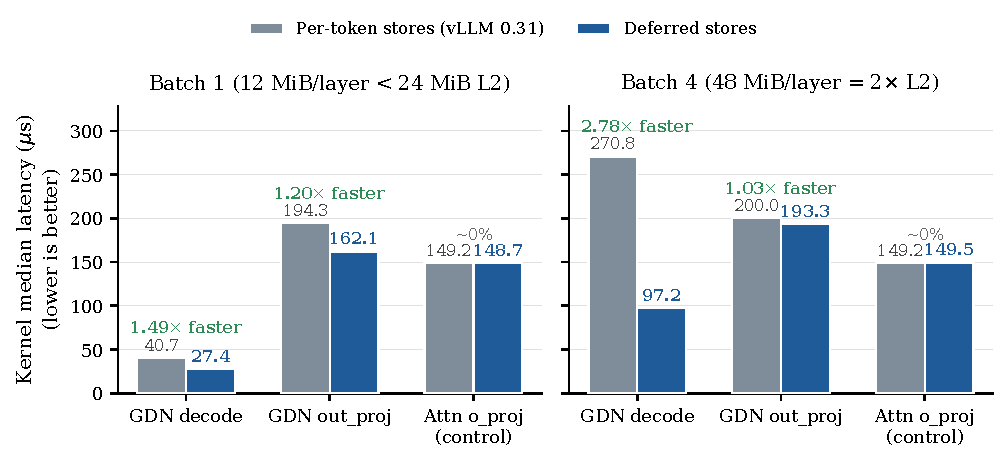
\includegraphics[width=0.85\linewidth]{figures/per_kernel_ab}
\caption{Per-kernel medians with per-token and deferred stores. At batch 1 the saving appears in the next GEMM; at batch 4 in the GDN kernel itself.}\label{fig:ab}
\end{figure}

\subsection{Upstream}

We reported the issue~\cite{vllmissue69152} and ported the deferred stores to vLLM main on top of the
Triton change, which is still in review~\cite{vllmpr69160}. Both arms below therefore run main with
both changes applied. On main the CUDA kernel writes its records in the Triton
kernel's layout, one record per 16-row V block, so that a request can move between the fused CUDA
op and the Triton speculative path from one step to the next. That costs some speed against our
prototype (116 instead of 97\,\textmu s for the GDN kernel at batch 4). \Cref{tab:upstream} gives the end-to-end result on the same machine. The baseline is not
vLLM main itself but the same build with a local switch, not part of the PR, that turns off
\texttt{defer\_gdn\_spec\_state}, so that the fused CUDA kernel stores the state after every token
as before; both arms run the same code path otherwise. Serving throughput improves by 5.2\% at concurrency 4
and 7.5\% at concurrency 8, greedy tokens are identical in every decode-step run, and GSM8K
accuracy is unchanged.

\begin{table}[t]
\centering\small
\begin{tabular}{@{}lrrr@{}}
\toprule
 & per-token stores & deferred & change \\
\midrule
Decode step, batch 1 (GPU busy) & 120.00 / 119.85\,ms & 117.95 / 117.90\,ms & $-1.7\%$ \\
Decode step, batch 4 (GPU busy) & 132.22 / 132.94\,ms & 125.35 / 125.74\,ms & $-5.3\%$ \\
\texttt{vllm bench serve}, concurrency 1 & 27.14\,tok/s & 27.50\,tok/s & $+1.3\%$ \\
\texttt{vllm bench serve}, concurrency 4 & 94.48\,tok/s & 99.42\,tok/s & $+5.2\%$ \\
\texttt{vllm bench serve}, concurrency 8 & 164.18\,tok/s & 176.56\,tok/s & $+7.5\%$ \\
GSM8K, 200 questions, greedy & 0.975 & 0.975 & \\
\bottomrule
\end{tabular}
\caption{vLLM main with the deferred-store change, with deferral turned off by a local switch (per-token stores) and on (deferred).}\label{tab:upstream}
\end{table}

\subsection{A prediction from the books: smaller draft heads}\label{sec:drafthead}

The books also price the repeated \texttt{lm\_head} reads: each draft step streams the full
248k-vocabulary head, 5.6\,ms, 16.8\,ms per step for the three. Drafts only propose tokens and the main model checks them, so a draft head over part of the vocabulary can cost acceptance but never correctness. This is not a new idea: FR-Spec restricts drafting to a static list of frequent tokens~\cite{zhao2025frspec}, and the same has been proposed for MTP drafters in vLLM~\cite{vllmissue58578,vllmissue67220}. What we test here is the books' prediction of what it saves. We tried it in a replay of the vLLM recording (the same kernels at the same
addresses), replacing the drafts' \texttt{lm\_head} GEMM with an FP8 GEMV over the first 32\,768
token ids and filling the other columns with $-\infty$. This change exists only in the replay; it
is not part of vLLM.

\begin{table}[t]
\centering\small
\begin{tabular}{@{}lrr@{}}
\toprule
 & full vocabulary & first 32\,768 ids \\
\midrule
Step (median) & 120.4\,ms & 106.1\,ms \\
Greedy: tokens per step & 2.84 & 2.73 \\
Greedy: tokens/s & 23.6 & 25.7 ($+9\%$) \\
Sampled (3 seeds, $T$ 0.2 and 0.9): tokens per step & 2.51 & 2.49 \\
Sampled: tokens/s & 20.7 & 23.4 ($+13\%$) \\
\bottomrule
\end{tabular}
\caption{Draft heads over the full vocabulary and over its first 32\,768 ids, in the replay; batch 1, 200 tokens per request, one English prompt. Greedy output is identical.}\label{tab:drafthead}
\end{table}

The step lost 14.3 of the 16.8\,ms the books predicted; the rest is the GEMV and the $-\infty$
fill (\cref{tab:drafthead}). Greedy output is identical, as it must be, and acceptance drops a
little where the best draft lies outside the first 32\,768 ids, for a net gain of 9\% in greedy and
13\% in sampled decoding. Choosing the rows by token frequency in GSM8K, Python sources and English
documentation did no better. The measurement covers one English prompt at batch 1; the low ids
are mostly English pieces, so other languages may lose more acceptance, and larger batches were not measured. Upstream measurements confirm the concern: a static 32k
list loses 33\% of the acceptance length on multilingual prompts, and choosing additional rows per
draft token from the hidden state wins most of it back~\cite{vllmissue67220}.

\subsection{What \sys{} reports}

Run on the unmodified engine, \sys{} produces the out\_proj/o\_proj split with its 2.27\,ms per
step and names \texttt{gdn\_decode\_post\_conv\_mtp} as the last cache-touching kernel before every
slow launch, without being told where to look: its only model-specific input is the memory map. It also reports the repeated \texttt{lm\_head}
reads. It does not explain the split; the isolation and probe experiments above do. What it
removes is the search: the hand analysis needed traces, weight-size arithmetic and source
reading to get to the same table.
